%% ΣΧΕΔΙΑΣΗ & ΥΛΟΠΟΙΗΣΗ
%% Σε αυτό το κεφάλαιο περιγράφεται η διαδικασία σχεδίασης και 
%% υλοποίησης της εφαρμογής. Αναλύονται οι επιλογές που έχουν 
%% γίνει και με ποιόν τρόπο λειτουργούν κάποια βασικά τμήματα 
%% του κώδικα.

\chapter{Σχεδίαση \& Υλοποίηση}
Σε αυτό το κεφάλαιο γίνεται ανάλυση του συστήματος στα επιμέρους μέρη που το απαρτίζουν και περιγράφεται η διαδικασία της υλοποίησης τους. Επεξηγούνται τα σημαντικότερα σημεία στον κώδικα και οι αλγόριθμοι που χρησιμοποιούνται για την επίλυση των κυριότερων λειτουργιών. Έχουν συμπεριληφθεί τμήματα κώδικα αλλά και διαγράμματα τα οποία βοηθούν στην κατανόηση των λύσεων που επιλέχθηκαν για την ολοκλήρωση της εφαρμογής.

\begin{figure}[ht!]
\centering
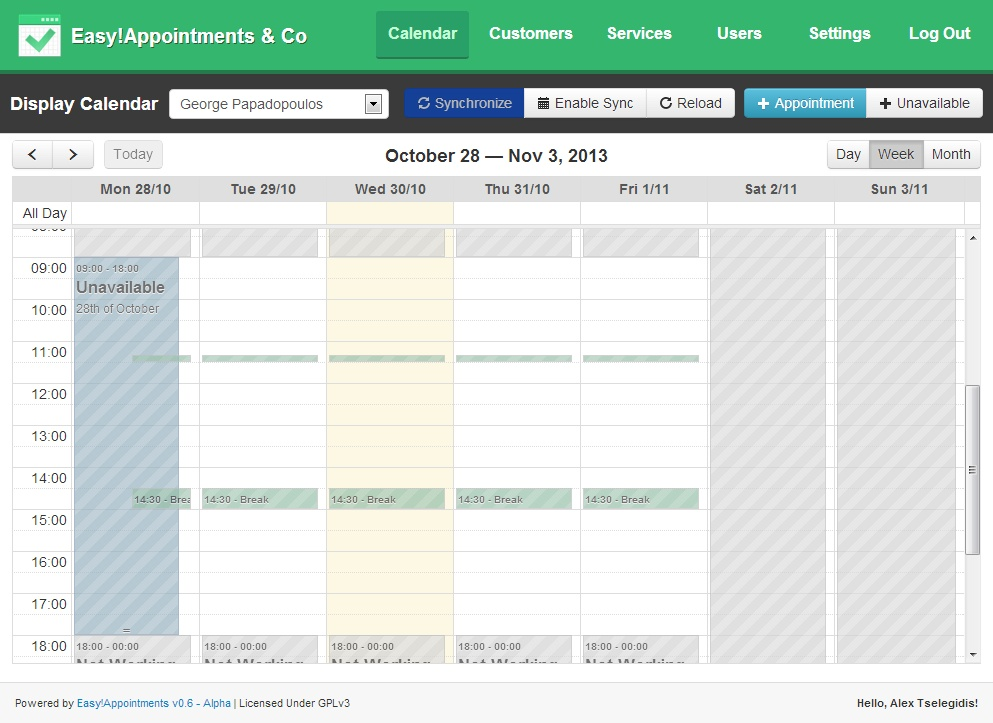
\includegraphics[width=130mm]{images/backend-calendar.jpg}
\caption{Σελίδα διαχείρισης ραντεβού.}
\label{backend-calendar}
\end{figure}

\begin{figure}[ht!]
\centering
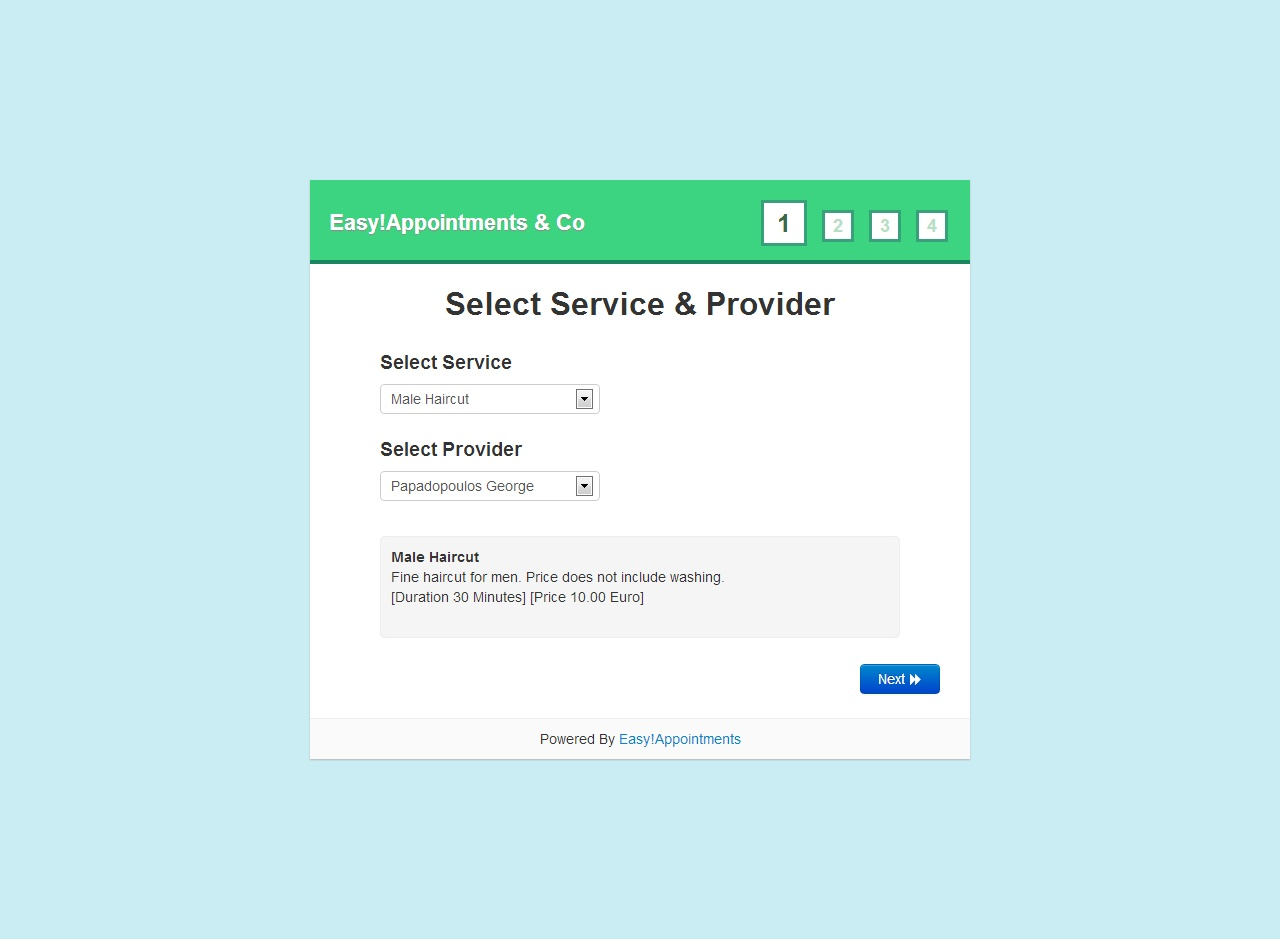
\includegraphics[width=130mm]{images/book-appointment.jpg}
\caption{Σελίδα κράτησης ραντεβού.}
\label{book-appointment}
\end{figure}

%% ================================================== 
%% ΑΝΑΛΥΣΗ ΔΕΔΟΜΕΝΩΝ
%% ==================================================
\section{Ανάλυση δεδομένων}
Το κυριότερο πρόβλημα που προσπαθεί να λύσει το σύστημα είναι η κράτηση και η διαχείριση ραντεβού από μια επιχείριση. Σε αυτήν την περίπτωση χρήσης έχει επικεντρωθεί η σχεδίαση και η υλοποίηση του συστήματος το οποίο περιέχει και άλλες δυνατότητες οι οποίες μπορούν όμως να θεωρηθούν λιγότερο σημαντικές. Έχοντας υπόψιν την έννοια "ραντεβού" ως την κύρια οντότητα της εφαρμογής, σχεδιάστηκε το παρακάτω μοντέλο το οποίο διευκρινίζει τις σχέσεις των οντοτήτων του συστήματος μεταξύ τους.

\begin{figure}[ht!]
\centering
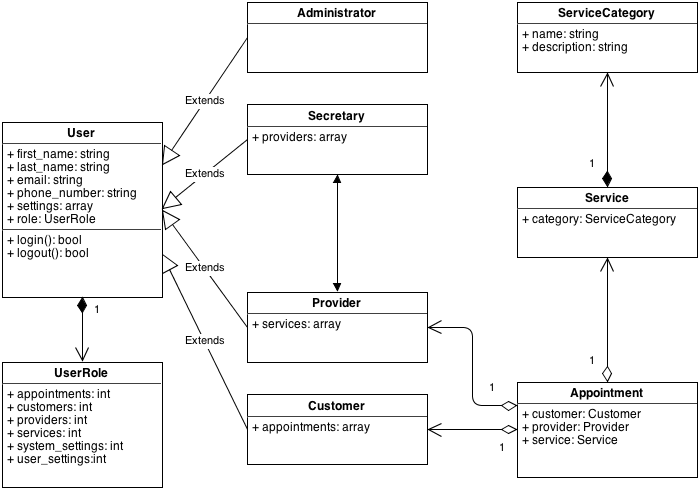
\includegraphics[width=160mm]{images/domain-model.png}
\caption{Domain model του συστήματος.}
\label{domain-model}
\end{figure}

Με βάση αυτό το σχεδιάγραμμα μπορεί πολύ εύκολα να προκύψει και το σχεδιακό μοντέλο της βάσης δεδομένων, δεδομένου ότι έχουμε τις οντότητες αλλά και τις σχέσεις μεταξύ τους. Όλοι οι χρήστες κληρονομούν την συμπεριφορά τους από μια οντότητα (User) και επιπρόσθετα κατέχουν διάφορες ιδιότητες που είναι αναγκαίες για τον ρόλο τους μέσα στην εφαρμογή. Για παράδειγμα ο χρήστης γραμματέας (Secretary) περιέχει έναν πίνακα από πάροχους (Providers) τους οποίους μπορεί να διαχειριστεί όπως και ένα ραντεβού είναι ξεκάθαρο ότι περιέχει στην πληροφορία του έναν πελάτη, έναν πάροχο και μια υπηρεσία.

\begin{figure}[ht!]
\centering
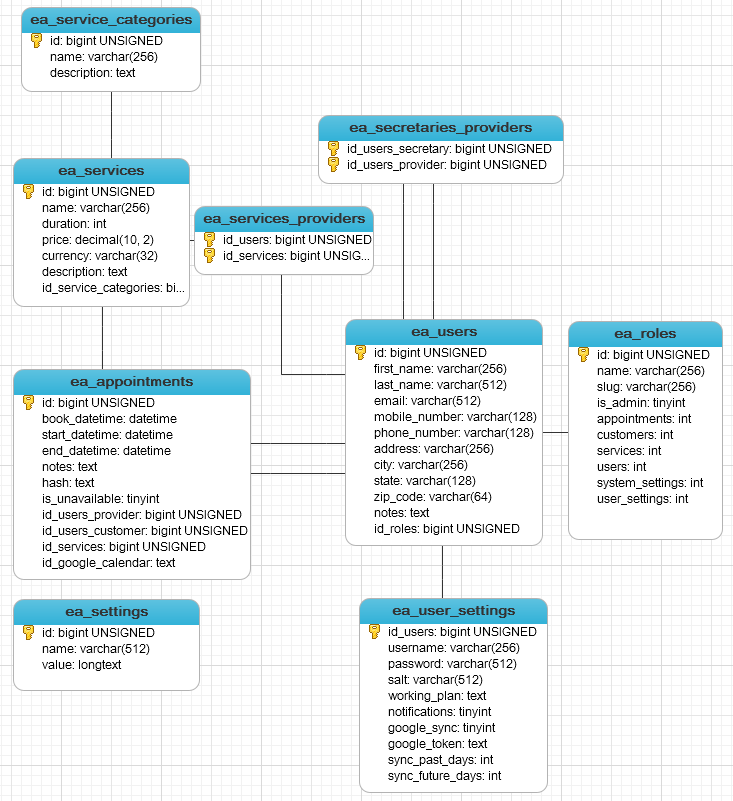
\includegraphics[width=160mm]{images/er.png}
\caption{Σχεσιακό μοντέλο της βάσης δεδομένων (ER).}
\label{er}
\end{figure}

Για την διαχείριση των δεδομένων της βάσης δημιουργήθηκαν ειδικές κλάσεις (models) οι οποίες περιέχουν μεθόδους που χρησιμοποιούνται από τους controllers του συστήματος. Το CodeIgniter δίνει στον προγραμματιστή ένα δικό του μέσο επικοινωνίας με την βάση δεδομένων, το οποίο είναι ένα πολύ ισχυρό και ευέλικτο εργαλείο. Η επονομαζόμενη Database Class του CodeIgniter επιτρέπει στον προγραμματιστή να εκτελεί ερωτήματα προς την βάση, να παράγει αποτελέσματα και να τα αναλύει σε ξεχωριστές εγγραφές, να κρατάει στην μνήμη ερωτήματα για γρηγορότερη ανταπόκριση (query caching) και κυριότερο την κλάση Active Record. Η κλάση αυτή έχει έναν δικό της τρόπο για την εκτέλεση των ερωτημάτων προς την βάση. Όλα τα τμήματα ενός τυπικού ερωτήματος είναι μέθοδοι οι οποίες χρησιμοποιούνται από τον προγραμματιστή ως το μέσο επικοινωνίας με την βάση δεδομένων. Το θετικό είναι ότι ανεξαρτήτως τον τύπο της βάσης η κλάση αυτή λειτουργεί με τον ίδιο τρόπο (MySQL, PostgreSQL, MSSQL κτλ). Η τεχνική αυτή λέγεται Active Record Database Pattern και έχει να κάνει με την αλλαγή adapter στην κλάση ανάλογα με τον τύπο της βάσης. Σε κάθε περίπτωση όμως ο τρόπος χρήσης της Active Record Class είναι ο ίδιος. Στο παρακάτω τμήμα κώδικα αναφέρεται ένα παράδειγμα για το πως μπορεί να βρεθεί το αναγνωριστικό μιας εγγραφής χρησιμοποιώντας ως κλειδί την διεύθυνση email.

\lstinputlisting{snippets/find_record_id.php}

%% ================================================== 
%% ΑΡΧΙΤΕΚΤΟΝΙΚΗ ΚΩΔΙΚΑ
%% ==================================================
\section{Αρχιτεκτονική κώδικα}
Η εφαρμογή είναι γραμμένη χρησιμοποιώντας τις εξής τεχνολογίες: PHP, Javascript, HTML, CSS, MySQL. Εκτός αυτών έχουν χρησιμοποιηθεί και κάποια βοηθητικά εργαλεία τα οποία διευκολύνουν τον προγραμματιστή στο να πετύχει καλύτερο αποτέλεσμα σε μικρότερο χρόνο. Αυτά τα εργαλεία (frameworks) όπως έχουν αναφερθεί και σε προηγούμενο κεφάλαιο είναι τα CodeIgniter (PHP), jQuery (JavaScript), Bootstrap (CSS + JavaScript). 

Όσον αφορά την αρχιτεκτονική του κώδικα έχει επιλεχθεί το μοντέλο MVC (Model - View - Controller) το οποίο υλοποιείται με άριστη απόδοση και οργάνωση χάρη στο framework CodeIgniter. Ο κώδικας PHP έχει χωριστεί σε τρία μέρη (models, views, controllers) και με αυτόν τον τρόπο παραμένει σε όλο τον κώδικα της εφαρμογής. Ο διαχωρισμός αυτός βελτιώνει τις συνθήκες συντήρησης γιατί είναι ξεκάθαρο σε ποιο από τα τρία ξεχωριστά σημεία ανήκει μια λειτουργία, όταν αυτή αναζητείται από τον προγραμματιστή. Έχουν συγγραφεί και δοκιμαστεί κλάσεις models για κάθε οντότητα οι οποίες αναλαμβάνουν την διαχείριση των δεδομένων με την βάση και παρέχουν μεθόδους που επαναχρησιμοποιούνται σε διάφορες περιπτώσεις. Επίσης έχουν δημιουργηθεί views για κάθε σελίδα που μπορεί να δει ο χρήστης τα οποία συνδέονται με ένα κομμάτι CSS κώδικα, υπεύθυνο για την μορφοποίησή τους. Τέλος τον συντονισμό αυτών των τμημάτων αναλαμβάνουν οι κλάσεις controllers οι οποίες είτε είναι υπεύθυνες για την σωστή φόρτωση μιας σελίδας της εφαρμογής, είτε απαντούν σε κλήσεις της JavaScript που γίνονται μέσω της τεχνολογίας AJAX.

Πολύ μεγάλο μέρος της εφαρμογής έχει γραφεί σε JavaScript για να μπορέσει το περιβάλλον εργασίας του χρήστη να γίνει αρκετά φιλικό και λειτουργικό. Ο JavaScript κώδικας χωρίζεται σε διάφορες κλάσεις και namespace τα οποία χρησιμοποιούνται από μια ή και παραπάνω σελίδες και στόχο έχουν να "ζωντανέψουν" το περιεχόμενο προσθέτοντας διαδραστικότητα. Πολλές φορές είναι απαραίτητο να εκτελεστούν κλήσεις AJAX προς τον server για την λήψη πρόσθετων πληροφοριών, είτε για να αποσταλούν δεδομένα τα οποία σηματοδοτούν για παράδειγμα κάποια επεξεργασία ή και διαγραφή εγγραφής από την βάση δεδομένων. Η χρήση του AJAX κρίνεται σημαντική διότι με αυτήν αποφεύγονται οι συνεχείς επαναφορτώσεις των σελίδων, οι οποίες θα γινόταν για να μπορέσει ο client να επικοινωνήσει με τον server. Αυτό το κομμάτι αναλαμβάνεται εξ ολοκλήρου από την JavaScript και προσδίδει ευελιξία και ταχύτητα στην χρήση της εφαρμογής. Το framework jQuery αποτελεί σημαντικό εργαλείο για την διεκπεραίωση διαφόρων λειτουργιών μέσω της JavaScript διότι δίνει την δυνατότητα στον προγραμματιστή να γράψει κώδικα όμορφα δομημένο και πολύ πιο αποδοτικό από ότι θα ήταν χωρίς την χρήση του. Αυτή η ιδιότητα της βιβλιοθήκης συντελεί και στην δημοτικότητά της και την χρήση της από κολοσσούς ανάπτυξης λογισμικού.

Για την μορφοποίηση των σελίδων της εφαρμογής χρησιμοποιήθηκε το πιο διαδεδομένο CSS framework την συγκεκριμένη την περίοδο, το Bootstap. Χρησιμοποιώντας αυτό το framework γράφτηκε νέο CSS το οποίο μορφοποιεί τις σελίδες έτσι ώστε να ανταποκρίνονται όπως πρέπει σε διάφορα μεγέθη οθονών, ενώ παράλληλα δεν χαλάει την συμβατότητα μεταξύ των διάφορων περιηγητών διαδικτύου. Το Bootstrap περιέχει και κάποια πρόσθετα JavaScript τα οποία βοηθούν σημαντικά στο οπτικό αποτέλεσμα της διεπαφής χρήστη.

Στο παρακάτω σχεδιάγραμμα γίνεται σαφής ο διαχωρισμός του κώδικα του συστήματος στα διάφορα τμήματα που το απαρτίζουν και η χρήση των εξωτερικών εργαλείων που συντέλεσαν στην ορθή ανάπτυξη της εφαρμογής.

\begin{figure}[ht!]
\centering
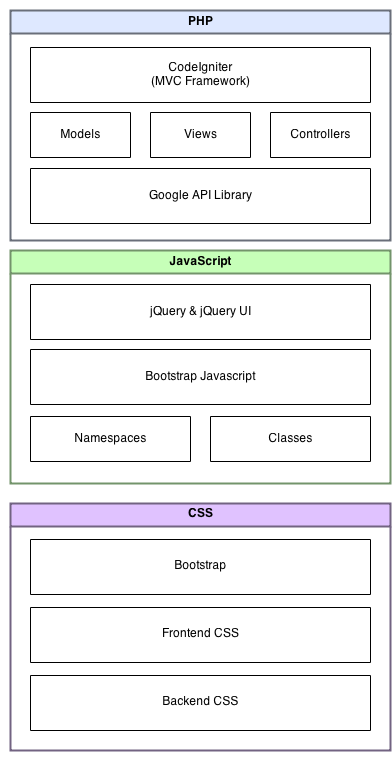
\includegraphics[width=100mm]{images/system-architecture.png}
\caption{Τα τμήματα που απαρτίζουν το Easy!Appointments.}
\label{system-architecture}
\end{figure}

%% ================================================== 
%% ΥΛΟΠΟΙΗΣΗ ΣΥΣΤΗΜΑΤΟΣ
%% ==================================================
\section{Υλοποίηση συστήματος}
Εφόσον ο αρχικός σχεδιασμός είχε ολοκληρωθεί ξεκίνησε η υλοποίηση της εφαρμογής με πρώτη εργασία τον σχεδιασμό της βάσης δεδομένων. Έχοντας ήδη σχεδιασμένο το domain model η δημιουργία του σχήματος της βάσης έγινε γρήγορα και διατηρήθηκε ως την ολοκλήρωση του έργου με μικρές προσθήκες όπου ήταν απαραίτητο. 

Στην συνέχεια, πριν γραφεί κώδικας θα έπρεπε να γίνει η επιλογή και το στήσιμο των εξωτερικών βιβλιοθηκών που θα κρίνονταν απαραίτητα για την λειτουργία του συστήματος. Σε αυτήν την φάση επιλέχθηκαν οι βασικές βιβλιοθήκες (CodeIgniter, Google API Library, jQuery, Bootstrap) καθώς και η σημαντικότερη περίπτωση χρήσης για να υλοποιηθεί πρώτη. Αυτή δεν ήταν άλλη από την κράτηση ενός ραντεβού από τον πελάτη. Αυτή η απόφαση πάρθηκε γιατί με αυτόν τον τρόπο θα καθορίζονταν εν μέρη και η αρχιτεκτονική του συστήματος καθώς αυτό θα εξελισσόταν σταδιακά με την ολοκλήρωση και των υπόλοιπων περιπτώσεων χρήσης.

Η κύρια ροή εργασιών ως προς την υλοποίηση μιας περίπτωσης χρήσης αποτελείται από τα παρακάτω βήματα:
\begin{enumerate}
\item Συγγραφή της κλάσης model για την συγκεκριμένη οντότητα. Μερικές φορές αυτή η διαδικασία μπορεί να συμπεριλάμβανε και την δημιουργία model και για άλλες οντότητες που εμπλέκονταν στην περίπτωση χρήσης, έτσι ώστε να μπορέσει να λειτουργήσει σωστά ο κώδικας συνολικά. Οι περισσότερες κλάσεις ακολουθούν το ίδιο πρότυπο σχεδίασης και μεθόδων με μικρές διαφοροποιήσεις ανάλογα με την οντότητα που διαχειρίζονται. 
\item Έλεγχος των model με δημιουργία unit tests. Μετά την ολοκλήρωση των model αυτά θα έπρεπε να δοκιμαστούν έτσι ώστε να διασφαλιστεί η σωστή λειτουργία τους. Εκτός αυτού όμως η συγγραφή unit test είναι και μια καλή ευκαιρία ως παράδειγμα της χρήσης των model από το υπόλοιπο σύστημα. Αν εντοπιζόταν κάποιο πρόβλημα κατά την εκτέλεση των test αυτό διορθωνόταν και τα test εκτελούνταν πάλι έως ότου να ολοκληρωθούν όλα με επιτυχία.
\item Εφόσον τα model ήταν ολοκληρωμένα στην συνέχεια δημιουργήθηκαν οι controllers και οι αντίστοιχες συναρτήσεις που θα ήταν υπεύθυνες για την λειτουργία του view που αντιστοιχούσε στην εκάστοτε περίπτωση χρήσης. Έτσι εκτός από τις συναρτήσεις που αναλάμβαναν να φορτώσουν μια σελίδα της εφαρμογής συγκεντρώνοντας τα δεδομένα που ήταν απαραίτητα, υλοποιήθηκαν και οι κλήσεις AJAX που ήταν απαραίτητες από την JavaScript. Αυτές οι κλήσεις συνήθως αναλάμβαναν την διεκπεραίωση κάποιας ενέργειας προς την βάση δεδομένων και επέστρεφαν πάντα κάποιο αποτέλεσμα για να μπορέσει να συνεχίσει την λειτουργία της το τμήμα της JavaScript.
\item Στην συνέχεια υλοποιούνταν το αντίστοιχο view που θα έβλεπε ο χρήστης. Σε αυτό τοποθετούνταν ο κώδικας PHP, HTML και η μορφοποίηση της σελίδας (CSS) γραφόταν στο αντίστοιχο αρχείο έτσι ώστε να παραχθεί ένα καλαίσθητο και φιλικό αποτέλεσμα.
\item Όταν το view ήταν έτοιμο θα έπρεπε να του προστεθεί και κάποια λειτουργικότητα έτσι ώστε να μπορεί να ανταποκριθεί στις ενέργειες του χρήστη. Για κάθε σελίδα χρησιμοποιούνται μια πληθώρα από βιβλιοθήκες, namespaces, κλάσεις και πρόσθετα JavaScript. Στα αντίστοιχα αρχεία τοποθετήθηκε ο κώδικας που θα ρύθμιζε την λειτουργία της σελίδας και τις ασύγχρονες κλήσεις προς τον server (AJAX). 
\item Τέλος εφόσον όλα ήταν έτοιμα και η περίπτωση χρήσης είχε υλοποιηθεί χωρίς προβλήματα, όλος ο κώδικας που είχε γραφεί έπρεπε να εξεταστεί (review) για τυχόν προβλήματα λογικής και για την βελτίωση της απόδοσης του, μικραίνοντας όσο είναι δυνατόν την σύζευξη και αυξάνοντας την συνοχή.
\end{enumerate}

Εδώ θα χρειαστεί να αναφερθεί ότι όλες οι κλήσεις AJAX που αφορούν το backend έχουν μεταφερθεί σε μια κλάση controller ξεχωριστά από τον κύριο controller του backend για να είναι καλύτερα οργανωμένες. Αν μελλοντικά ο αριθμός τους και η πολυπλοκότητα τους αυξηθεί τότε θα χρειαστεί να διαιρεθούν ξανά για να μπορέσουν να συντηρούνται πιο εύκολα.

%% ================================================== 
%% ΠΕΡΙΓΡΑΦΗ ΒΑΣΙΚΩΝ ΑΛΓΟΡΙΘΜΩΝ
%% ==================================================
\section{Περιγραφή βασικών αλγορίθμων}
Σε αυτήν την ενότητα θα γίνει ανάλυση κάποιων βασικών αλγορίθμων που αποτελούν κρίσιμα τμήματα για την λειτουργία του συστήματος. Η περιγραφή θα γίνει σχολιάζοντας τα τμήματα κώδικα που απαρτίζουν αυτούς τους αλγορίθμους αναφέροντας και τις συγκεκριμένες γραμμές στα οποία αναφέρονται. Στην επόμενη ενότητα παρέχονται κάποια σχεδιαγράμματα τα οποία μπορούν να βοηθήσουν στην κατανόηση αυτών των αλγορίθμων.

\subsection{Πλήρης συγχρονισμός με το Google Calendar}
Η διαδικασία του πλήρη συγχρονισμού των ραντεβού με το Google Calendar αποτελεί ένας από τους κυριότερους αλγορίθμους του Easy!Appointments. Η πολυπλοκότητα της διαδικασίας συγχρονισμού δεδομένων κατέστησαν την υλοποίηση αυτού του τμήματος κώδικα αρκετά ενδιαφέρον και το αποτέλεσμα κατάφερε να καλύψει τις αρχικές απαιτήσεις. Μπορεί μελλοντικά να υπάρξουν βελτιώσεις στον κώδικα αλλά την συγκεκριμένη στιγμή ο αλγόριθμος λειτουργεί επιτυχώς και συγχρονίζει τα ραντεβού του συστήματος με τα συμβάντα που έχει περάσει ο χρήστης στο Google Calendar.

\lstinputlisting{snippets/google_sync_algorithm.php}

Η μέθοδος αυτή καλείται κάθε φορά που πρέπει να τρέξει ο αλγόριθμος συγχρονισμού για έναν πάροχο υπηρεσιών. Στο πρώτο μέρος του κώδικα ελέγχεται αν ο χρήστης έχει τα δικαιώματα να τρέξει αυτήν την μέθοδο και αν έχει δοθεί το αναγνωριστικό της εγγραφής του πάροχου. Έπειτα φορτώνονται τα απαραίτητα models και γίνεται η λήψη των πληροφοριών του πάροχου από την βάση (γραμμές 17 - 30). 

Για να συνεχιστεί η διαδικασία θα πρέπει να ελεγχθεί αν ο πάροχος έχει ενεργό τον συγχρονισμό με το Google Calendar. Αν η επιλογή αυτή είναι ενεργή τότε ο αλγόριθμος χρησιμοποιεί το token του πάροχου για να πιστοποιήσει την χρήση των δεδομένων του στο Google Calendar, διαφορετικά η διαδικασία τερματίζεται (γραμμές 33 - 43). 

Για να γίνει εξοικονόμηση κλήσεων προς την υπηρεσία της Google αλλά και να μειωθεί ο χρόνος διεκπεραίωσης του αλγορίθμου συγχρονισμού, το χρονικό διάστημα μέσα στο οποίο θα συγχρονισθούν τα δεδομένα περιορίζεται στο εύρος ημερών που έχει τεθεί ως ρύθμιση για τον κάθε πάροχο (προεπιλεγμένη τιμή 5 ημέρες στο παρελθόν και 5 στο μέλλον). Αυτό είναι το χρονικό διάστημα στο οποίο θα ελεγχθούν όλα τα δεδομένα και από τα δύο συστήματα και θα συντονιστούν έτσι ώστε να είναι τα ίδια (γραμμές 47 - 54).

Το επόμενο κομμάτι κώδικα αφού πρώτα λάβει τα ραντεβού από την βάση δεδομένων του Easy!Appointments, εξετάζει τις εγγραφές μια προς μια για το αν έχουν συγχρονιστεί με το Google Calendar. Εδώ υπάρχουν οι εξής περιπτώσεις:
\begin{enumerate}
\item Το ραντεβού δεν έχει ακόμα συγχρονιστεί οπότε θα πρέπει να προστεθεί στο Google Calendar (γραμμές 88 - 93).
\item Το ραντεβού είναι συγχρονισμένο και πρέπει να ελεγχθεί αν υπάρχουν διαφορές με το συμβάν που είναι καταχωρημένο στο Google Calendar. Αν ναι τότε αυτό σημαίνει ότι ο χρήστης έχει αλλάξει τα στοιχεία του συμβάντος στο Google Calendar και η εγγραφή του ραντεβού στο Easy!Appointments θα πρέπει να ενημερωθεί (γραμμές 97 - 126).
\item Το ραντεβού είναι συγχρονισμένο αλλά δεν έχει βρεθεί στο Google Calendar. Εφόσον δεν έχει βρεθεί η εγγραφή σημαίνει ότι ο χρήστης την έχει διαγράψει από το Google Calendar και έτσι θα πρέπει να διαγραφεί και από το Easy!Appointments (γραμμές 130 - 131).
\end{enumerate}
Με το πέρας αυτού του τμήματος κώδικα όλα τα ραντεβού του Easy!Appointments θα πρέπει να έχουν συγχρονιστεί με το Google Calendar.

Τα μη διαθέσιμα διαστήματα χρησιμοποιούνται ως ραντεβού στον συγκεκριμένο αλγόριθμο με την διαφορά ότι δεν υπάρχουν σε αυτά πληοροφίες για κάποιο πελάτη ή υπηρεσία (γραμμές 83 - 84).

Υπάρχουν όμως συμβάντα στην υπηρεσία της Google τα οποία μπορεί να έχουν προστεθεί απευθείας στο Google Calendar και να μην υπάρχουν στο Easy!Appointments. Σε αυτήν την περίπτωση θα πρέπει να ανιχνευθούν και να εξεταστούν όλα τα συμβάντα που αντιστοιχούν στην χρονική περίοδο συγχρονισμού (5 ημέρες πριν και 5 ημέρες μετά την τρέχουσα ημερομηνία) και να ελεγχθεί αν υπάρχει κάποιο συμβάν που δεν είναι συγχρονισμένο. 

Αυτήν την εργασία αναλαμβάνει το επόμενο κομμάτι κώδικα το οποίο χρησιμοποιώντας την βιβλιοθήκη Google API μπορεί να διαβάσει τα συμβάντα τα οποία βρίσκονται στο Google Calendar. Η διαδικασία ξεκινάει με την λήψη αυτών των συμβάντων τα οποία στην συνέχεια εξετάζονται ένα προς ένα για το αν υπάρχουν στο Easy!Appointments. Αν όχι τότε προστίθενται και συγχρονίζονται και στα δύο συστήματα και έτσι διασφαλίζεται η ακεραιότητα των δεδομένων και στα δύο συστήματα (γραμμές 137 - 159). 

Τέλος η συνάρτηση επιστρέφει την σταθερά AJAX\_SUCCESS την οποία θα διαβάσει η JavaScript και έτσι θα γνωρίζει ότι η διαδικασία έχει ολοκληρωθεί με επιτυχία. Διαφορετικά αν προκύψουν σφάλματα αυτά επιστρέφονται σε JSON μορφή και εμφανίζονται με ένα φιλικό μήνυμα προς τον χρήστη.

\subsection{Υπολογισμός διαθέσιμων ωρών πάροχου}
Ένα κομβικό σημείο στον κώδικα της εφαρμογής είναι ο υπολογισμός των διαθέσιμων ωρών ενός πάρoχου, στις οποίες μπορεί ένας πελάτης να κλείσει ένα ραντεβού για μια υπηρεσία, χωρίς να υπάρχει σύγκρουση με άλλα συμβάντα. Για να επιτευχθεί ο υπολογισμός αυτός χρειάζεται να γίνουν αρκετοί έλεγχοι έτσι ώστε τα αποτελέσματα να είναι σωστά και να μην δημιουργούνται προβλήματα με τα πλάνα των πάροχων υπηρεσιών. Η διαδικασία χωρίζεται σε δύο μεθόδους με την πρώτη να υπολογίζει τα ελεύθερα χρονικά διαστήματα του πάροχου και την δεύτερη να υπολογίζει τις ακριβείς ώρες στις οποίες θα μπορεί ο πελάτης να κλείσει ραντεβού.

\lstinputlisting{snippets/provider_available_periods.php}

Το πρώτο πράγμα που πρέπει να γίνει είναι η λήψη του πλάνου εργασίας του πάροχου καθώς και των ήδη καταχωρημένων ραντεβού για την επιλεγμένη ημερομηνία. Επίσης υπάρχει και η περίπτωση να πρέπει να αποκλειστούν κάποια ραντεβού κατά τον υπολογισμό των διαθέσιμων ωρών οπότε αν έχουν οριστεί τέτοιες εγγραφές δεν λαμβάνονται υπόψιν στον υπολογισμό. Αυτή η επιλογή είναι απαραίτητη όταν χρειάζεται ο πελάτης να επεξεργαστεί ένα ήδη καταχωρημένο ραντεβού το οποίο δεν θα πρέπει να εμφανίζει ως δεσμευμένη την ώρα που αντιστοιχεί στο ίδιο στο ημερολόγιο του πάροχου. Τα στοιχεία αυτά θα χρησιμοποιηθούν έτσι ώστε τα διαθέσιμα διαστήματα που θα υπολογιστούν να αντιπροσωπεύουν τον χρόνο στον οποίο ο πάροχος θα είναι διαθέσιμος (γραμμές 23 - 47).

Έπειτα θα διαχωριστούν τα ελεύθερα χρονικά διαστήματα του πάροχου από τα διαλείμματα και τα ήδη καταχωρημένα ραντεβού. Αρχικά για την επιλεγμένη ημέρα του ραντεβού ελέγχονται αν υπάρχουν καθόλου διαλείμματα. Αν ναι, τότε τα διαθέσιμα διαστήματα χωρίζονται μεταξύ των διαλειμμάτων του πάροχου (γραμμές 54 - 81) και παράγονται νέα χρονικά διαστήματα. Στην συνέχεια λαμβάνονται υπόψιν τα ραντεβού που έχουν ήδη κρατηθεί. Τα διαθέσιμα χρονικά διαστήματα του πάροχου θα διασπαστούν ξανά μεταξύ των ραντεβού αυτών και έτσι θα ολοκληρωθεί η διαδικασία του υπολογισμού (γραμμές 84 - 137). Αν την επιλεγμένη ημερομηνία ο πάροχος δεν έχει κανένα ραντεβού τότε δεν πραγματοποιείται καμία επιπλέον διάσπαση και το αποτέλεσμα επιστρέφεται όπως είναι. Στην επόμενη μέθοδο ο πίνακας που περιέχει τα διαστήματα θα χρησιμοποιηθεί για να υπολογιστούν οι ακριβείς διαθέσιμες ώρες στις οποίες θα μπορεί ο πελάτης να κλείσει κάποιο ραντεβού για την επιλεγμένη υπηρεσία.

\lstinputlisting{snippets/provider_appointment_hours.php}

Η δεύτερη μέθοδος αποτελεί απάντηση σε κλήση της JavaScript με χρήση της τεχνικής AJAX. Όταν ο client καλεί αυτήν την μέθοδο, παρέχει τα στοιχεία του πάροχου, την διάρκεια της επιλεγμένης υπηρεσίας (σε λεπτά) και το αν ο χρήστης επεξεργάζεται το συγκεκριμένο ραντεβού ή όχι (παράμετρος manage\_mode). Αυτό που εκτελείται αρχικά είναι η λήψη των ελεύθερων χρονικών διαστημάτων του πάροχου χρησιμοποιώντας την προαναφερθέντα μέθοδο get\_provider\_available\_time\_periods (γραμμές 28 - 34). 

Έπειτα θα υπολογιστούν οι διαθέσιμες ώρες στις οποίες θα μπορέσει ο πελάτης να κλείσει ραντεβού. Αυθαίρετα και για λόγους ευχρηστίας έχει τεθεί το χρονικό διάστημα μεταξύ των ελεύθερων ωρών να είναι τα 15 λεπτά. Αυτό που κάνει το συγκεκριμένο κομμάτι κώδικα είναι ουσιαστικά ο διαχωρισμός των ελεύθερων χρονικών διαστημάτων του πάροχου σε ώρες τις οποίες χωρίζουν 15 λεπτά τουλάχιστον και οι οποίες μπορούν να χωρέσουν την διάρκεια της υπηρεσίας για την οποία ενδιαφέρεται ο πελάτης, πριν την λήξη του διαθέσιμου χρονικού διαστήματος (γραμμές 41 - 74).

Στο τελευταίο μέρος αυτής της μεθόδου ελέγχεται αν η επιλεγμένη ημερομηνία αντιστοιχεί στην σημερινή και αν αυτό ισχύει αφαιρούνται οι παρελθοντικές διαθέσιμες ώρες έτσι ώστε να μην μπορεί ο πελάτης να κλείσει ραντεβού σε μια παρελθοντική χρονική στιγμή. Το σύστημα στο frontend δεν επιτρέπει ούτως ή άλλος την επιλογή παρελθοντικής ημερομηνίας, αλλά απαιτείται στην συγκεκριμένη περίπτωση να ελεγχθούν οι παρελθοντικές ώρες του ραντεβού. Επίσης είναι σημαντικό να αναφερθεί ότι η εφαρμογή παρέχει μια παράμετρο η οποία ορίζει το χρονικό διάστημα που θα πρέπει να χωρίζει ένα ραντεβού από την ώρα που αυτό γίνεται κράτηση ή επεξεργάζεται. Ο λόγος γίνεται για την ρύθμιση του συστήματος με το όνομα "book\_advance\_timeout" η οποία μετράται σε λεπτά και λαμβάνεται υπόψιν στον υπολογισμό των διαθέσιμων ωρών.

%% ================================================== 
%% ΔΙΑΓΡΑΜΜΑΤΑ ΚΩΔΙΚΑ
%% ==================================================
\section{Διαγράμματα Κώδικα}
Σε αυτήν την ενότητα θα παρατεθούν κάποια διαγράμματα κώδικα τα οποία θα βοηθήσουν τον αναγνώστη στην κατανόηση της λειτουργίας του συστήματος και στον τρόπο με τον οποίο διεκπεραιώνονται οι εργασίες που απαιτούνται στην εκάστοτε περίπτωση χρήσης. Τα διαγράμματα αυτά ακολουθούν το σχεδιαστικό πρότυπο UML το οποίο αποτελεί την πιο δημοφιλής γλώσσα μοντελοποίησης εδώ και αρκετά χρόνια.

Η εφαρμογή που χρησιμοποιήθηκε για τον σχεδιασμό των διαγραμμάτων αυτών είναι η draw.io και πρόκειται για μια διαδικτυακή πλατφόρμα με την οποία μπορούν να γίνουν σχεδιαγράμματα πολλών διαφορετικών τύπων. Το draw.io είναι δωρεάν προς χρήση και μπορεί να βρεθεί στην διεύθυνση http://www.draw.io.

\subsection{Διαγράμματα ροής}
Τα διαγράμματα ροής δείχνουν τον τρόπο και την σειρά με την οποία λειτουργούν οι διεργασίες και τα αντικείμενα μεταξύ τους για την διεκπεραίωση ενός σκοπού. Σε αυτά είναι εύκολο να διακριθούν ποιοι ηθοποιοί, αντικείμενα, διεπαφές και μέθοδοι αλληλεπιδρούν έτσι ώστε τα δεδομένα που χρειάζονται για την εργασία να παραχθούν επιτυχώς και να φτάσουν ακέραια στον προορισμό τους. Σε αυτά τα διαγράμματα ο χρονικός προσδιορισμός της κάθε αλληλεπίδρασης είναι εμφανής και πολύ σημαντικός για να μπορέσει ο προγραμματιστής να καταλάβει με ποια σειρά θα πρέπει να πορευτεί η εκτέλεση έτσι ώστε αυτός να καταλήξει σε αναμενόμενο αποτέλεσμα. Συνήθως τα διαγράμματα ροής συγχέονται με το σενάριο κάποιας περίπτωσης χρήσης αλλά μπορούν να διασπαστούν και σε μικρότερα τμήματα τα οποία να επικεντρώνουν στα σημεία που είναι πιο σημαντικά. 

\begin{figure}%% [Η] αυτή η εντολή θα τοποθετήσει το διάγραμμα ακριβώς σε αυτό το σημείο. Το latex όμως πάντα προσπαθεί να αφήσει όσο λιγότερα κενό χόρο γίνεται και έτσι τα διαγράμματα δεν θα εμφανιστούν με την σειρά που γράφονται στον κώδικα.
\centering
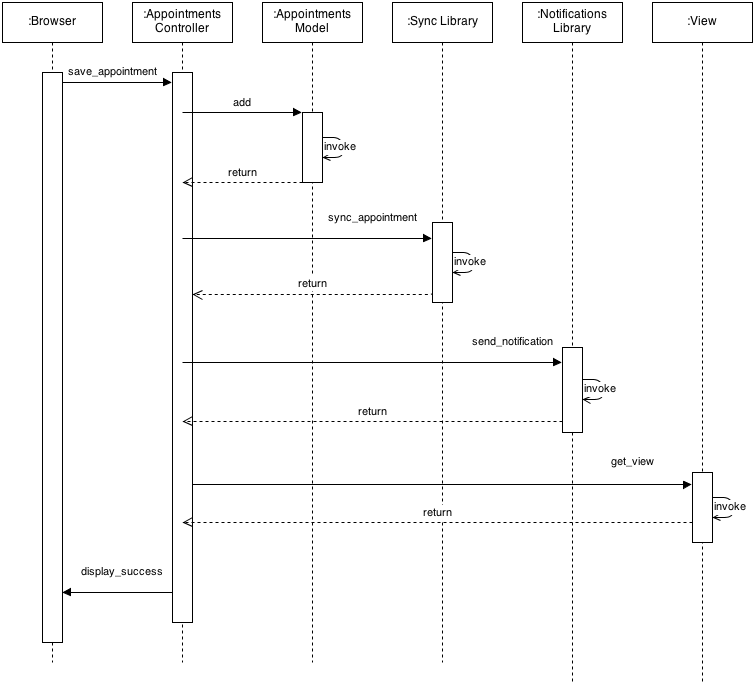
\includegraphics[width=150mm]{images/sd-save-appointment.png}
\caption{Διάγραμμα ροής για την διαδικασία αποθήκευσης ενός ραντεβού.}
\label{sd-save-appointment}
\end{figure}

\begin{figure}
\centering
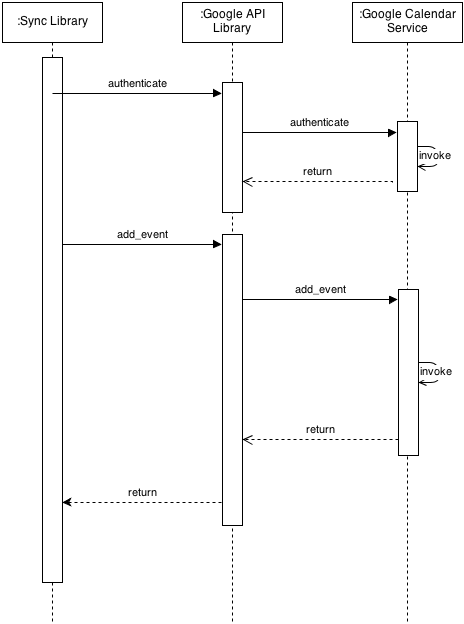
\includegraphics[width=150mm]{images/sd-sync-appointment.png}
\caption{Διάγραμμα ροής για την διαδικασία προσθήκης ενός ραντεβού στο Google Calendar.}
\label{sd-save-appointment}
\end{figure}

\subsection{Διαγράμματα δραστηριότητας}
Τα διαγράμματα δραστηριότητας αποτελούν γραφικές παρουσιάσεις της δραστηριότητας του που ακολουθεί το σύστημα ανάλογα με τις αποφάσεις που λαμβάνονται μέσα από τον κώδικα. Σε αυτά τα διαγράμματα μπορούν να φανούν τα σημεία στα οποία υπάρχουν βρόγχοι επανάληψης, τα σημεία όπου παίρνονται αποφάσεις όπως και επίσης τις διαδικασίες που τρέχουν ταυτόχρονα και σε ποιο σημείο χρονικά γίνεται αυτό. Κατά κύριο λόγο τα διαγράμματα δραστηριότητας δείχνει την συνολική ροή του ελέγχου μέσα από την εκτέλεση μιας συγκεκριμένης διαδικασίας. 

\begin{figure}
\centering
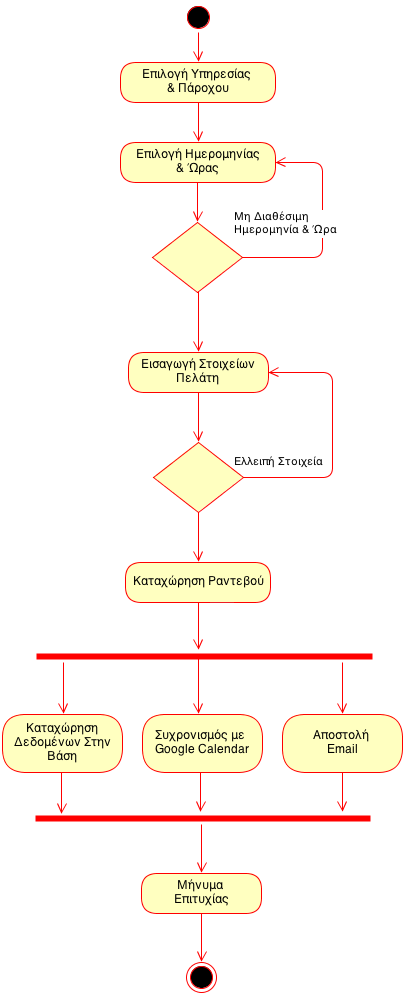
\includegraphics[width=90mm]{images/ad-book-appointment.png}
\caption{Διάγραμμα δραστηριότητας της διαδικασίας κράτησης ραντεβού.}
\label{ad-book-appointment}
\end{figure}

\begin{figure}
\centering
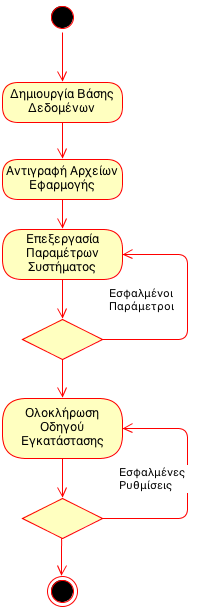
\includegraphics[width=70mm]{images/ad-install-application.png}
\caption{Διάγραμμα δραστηριότητας της διαδικασίας εγκατάστασης της εφαρμογής.}
\label{ad-install-application}
\end{figure}

\begin{figure}
\centering
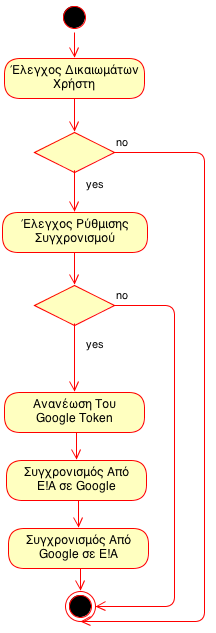
\includegraphics[width=70mm]{images/ad-sync-appointments.png}
\caption{Διάγραμμα δραστηριότητας της διαδικασίας αμφίδρομου συγχρονισμού με το Google Calendar.}
\label{ad-sync-appointments}
\end{figure}

\begin{figure}
\centering
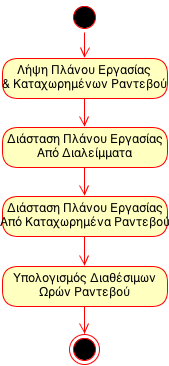
\includegraphics[width=70mm]{images/ad-provider-available-hours.png}
\caption{Διάγραμμα δραστηριότητας του υπολογισμού των διαθέσιμων ωρών ενός πάροχου.}
\label{ad-provider-available-hours}
\end{figure}

\subsection{Διαγράμματα κλάσεων}
Στην τεχνολογία λογισμικού, τα διαγράμματα κλάσεων περιγράφουν την στατική δομή ενός συστήματος δείχνοντας τις κλάσεις, τις ιδιότητες, τις λειτουργίες και τις σχέσεις μεταξύ των αντικειμένων. Τα σχεδιαγράμματα αυτά είναι τα βασικότερα για έναν προγραμματιστή διότι μπορεί άμεσα να πληροφορηθεί σχετικά με την δομή του κώδικα και με ποιόν τρόπο θα πρέπει να συνεχιστεί η διαδικασία της υλοποίησης. Επίσης είναι εμφανές και οι αρχιτεκτονικές επιλογές που έχουν γίνει καθώς κάθε σχεδιαστικό πρότυπο που πρέπει να έχει ο κώδικας μπορεί να διακριθεί και να περιγραφή σε αυτά τα διαγράμματα. Καλή πρακτική είναι πάντα ένα διάγραμμα να περιέχει μόνο την ουσία οπότε στο υποκεφάλαιο αυτό εμφανίζονται διαγράμματα κλάσης τα οποία δείχνουν κάποιες σχεδιαστικές επιλογές που έχουν γίνει στην εφαρμογή.

\begin{figure}
\centering
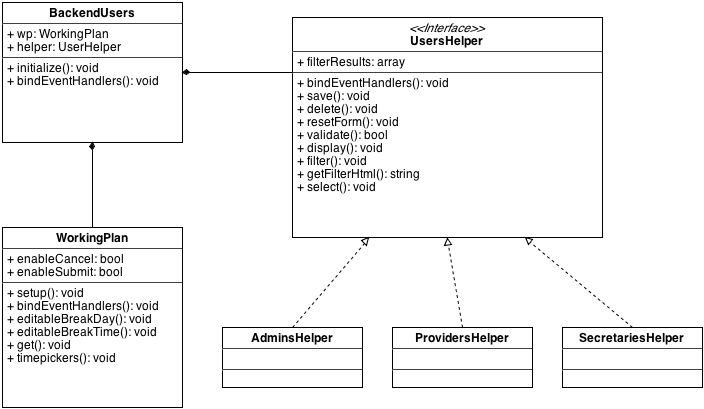
\includegraphics[width=150mm]{images/cd-backend-users.png}
\caption{Διάγραμμα κλάσεων της δομής JavaScript στην σελίδα διαχείρισης των χρηστών.}
\label{cd-backend-users}
\end{figure}

\begin{figure}
\centering
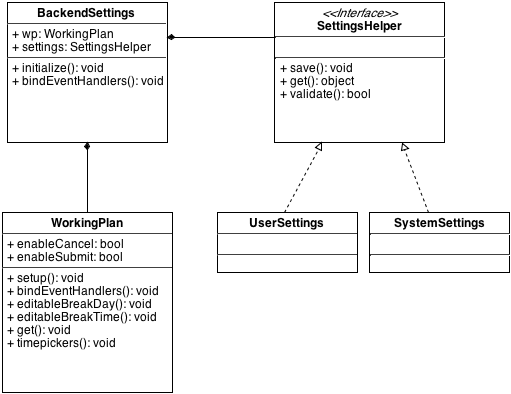
\includegraphics[width=150mm]{images/cd-backend-settings.png}
\caption{Διάγραμμα κλάσεων της δομής JavaScript στην σελίδα ρυθμίσεων της εφαρμογής.}
\label{cd-backend-settings}
\end{figure}
